\documentclass[tikz,border=10pt]{standalone}
\usepackage{amsmath}
\begin{document}
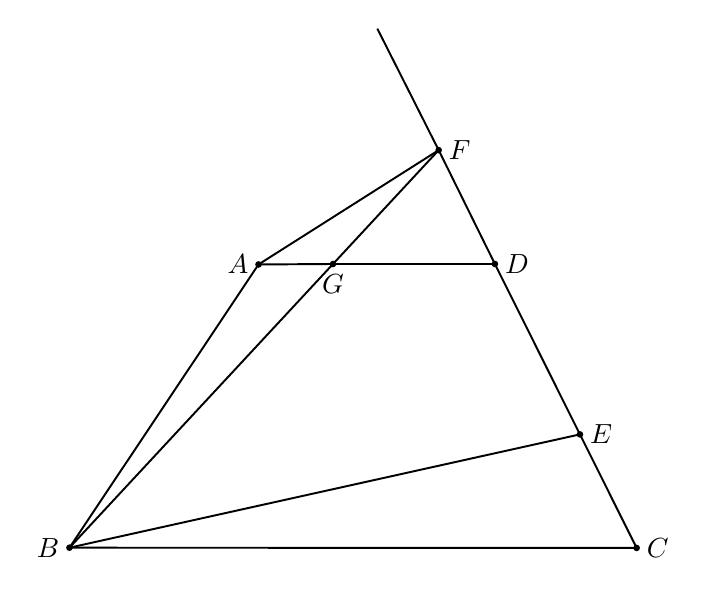
\begin{tikzpicture}[line width=0.7pt, line join=round]
\coordinate (A) at (-1.205,0.444);
\coordinate (B) at (-3.606,-3.153);
\coordinate (C) at (3.597,-3.156);
\coordinate (D) at (1.797,0.450);
\coordinate (E) at (2.877,-1.714);
\coordinate (F) at (1.083,1.896);
\coordinate (G) at (-0.259,0.450);











\coordinate (H) at (0.304,3.439);


\draw (C) -- (E);
\draw (E) -- (D);
\draw (D) -- (F);

\draw (F) -- (H);


\draw (B) -- (C);


\draw (A) -- (G) -- (D);


\draw (B) -- (G) -- (F);


\draw (A) -- (B);
\draw (A) -- (F);
\draw (B) -- (E);


\foreach \p in {A,B,C,D,E,F,G}
  \fill (\p) circle (1.200pt);


\node[left] at (A) {\fontsize{10}{12}\selectfont $A$};
\node[left] at (B) {\fontsize{10}{12}\selectfont $B$};
\node[right] at (C) {\fontsize{10}{12}\selectfont $C$};
\node[right] at (D) {\fontsize{10}{12}\selectfont $D$};
\node[right] at (E) {\fontsize{10}{12}\selectfont $E$};
\node[right] at (F) {\fontsize{10}{12}\selectfont $F$};
\node[below] at (G) {\fontsize{10}{12}\selectfont $G$};
\end{tikzpicture}
\end{document}